\documentclass[5pt]{article}
\usepackage{multicol,multirow}
\usepackage{graphicx} % Required for inserting images
\usepackage[margin=0.75cm]{geometry}
\usepackage{xcolor}
\usepackage{amsmath}
\usepackage{mathtools}
\usepackage{relsize}

\usepackage[english]{babel}
\newtheorem{theorem}{Theorem}

\usepackage{empheq}
\usepackage{amsfonts}

\usepackage{array}

\usepackage{tkz-euclide}
\usepackage{tikz}

\definecolor{LightGray}{gray}{0.9}

\usepackage{minted}

\DeclarePairedDelimiter\abs{\lvert}{\rvert}%
\DeclarePairedDelimiter\norm{\lVert}{\rVert}%

\makeatletter
\let\oldabs\abs
\def\abs{\@ifstar{\oldabs}{\oldabs*}}

\newcommand{\tr}[3]{
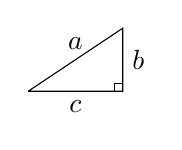
\begin{tikzpicture}[scale=0.40]
    \coordinate [] (A) at (-1.5cm,-1.cm);
    \coordinate [] (C) at (1.5cm,-1.0cm);
    \coordinate [] (B) at (1.5cm,1.0cm);
    \draw (A) -- node[above] {$a$} (B) -- node[right] {$b$} (C) -- node[below] {$c$} (A);
    \draw (1.25cm,-1.0cm) rectangle (1.5cm,-0.75cm);
\end{tikzpicture}
}


\begin{document}


\begin{center}
     \Large{\textbf{Python Programming}}\\
     \small{Class: COSC 1800}\hfill\small{\textcopyright Maximilien Notz \the\year{}}
     \noindent\rule{20.2cm}{0.4pt}
\end{center}


\begin{multicols}{2}
\setcounter{secnumdepth}{0}

\subsection{General Reminder}
\begin{tabular}{>{\ttfamily}l l}
    r.randint(x,y)      & Generate a random integer between \textbf{x}\\
                        & and \textbf{y}(import random as r).\\
    input(msg)          & Prompt the user with \textbf{msg} and take the\\
                        & user input.\\
    type(var)           & Returns the type of var.\\
    type(n, b, d,)      & Dynamicaly create a class named \textbf{n}.\\
                        & This class inerits all classes in \textbf{b} (tuple).\\
                        & \textbf{d} is a dictionary containing attributes\\
                        & and member method.\\
    int(var)            & Convert \texttt{var} to a integer.\\
    float(var)          & Convert \texttt{var} to a float.\\
    str(var)            & Convert \texttt{var} to a string.\\
    len(var)            & Returns the length of a string or a list.\\
    pass                & Used to keep an indentention empty\\
                        & avoiding \texttt{IndentationError}.\\
    .copy(obj)          & \\
    .deepcopy(obj)      & \\
\end{tabular}

\subsection{Basic Syntax}
\begin{minted}[bgcolor=LightGray]{Python}
    if conditon_1:
        # code if conditon_1 is true
    elif conditon_2:
        # code if conditon_2 is true and conditon_1 
        # is false
    else:
        # code
\end{minted}

\subsection{Lists}
\begin{minted}[bgcolor=LightGray]{Python}
    lst1 = [e_1, e_2, e_3] # [e_1, e_2, e_3]
    lst2 = 5 * [a] # [a, a, a, a, a]
    lst3 = [a for i in range(3)] # [a, a, a]
    print([1,3,5,7]) # [1, 3, 5, 7]
\end{minted}
\begin{tabular}{>{\ttfamily}l l}
    list(var)       & Convert a set or tuple to a list.\\
    lst[i]          & Access the \texttt{i}th element in the list.\\
    .apend(a)       & Adds \texttt{a} to the end of the list.\\
    .insert(i,e)    & Insert element \texttt{e} at index \texttt{i}.\\
    .pop()          & Remove the last element, return the \\
                    & removed value.\\
    .pop(i)         & Remove element at index \texttt{i}, return the \\
                    & removed value.\\
    range(i)        & \\
\end{tabular}


\subsection{Operators}
\begin{tabular}{|>{\ttfamily}l|l|l|}
    \hline
    Symbol  &   Name                    & Type       \\
    \hline
    +       & addition                  & Arithmetic \\
    -       & substraction              & Arithmetic \\
    *       & multiplication            & Arithmetic \\
    /       & division                  & Arithmetic \\
    \%      & modulo                    & Arithmetic \\
    **      & power                     & Arithmetic \\
    //      & div                       & Arithmetic \\
    and     & logical and               & Boolean    \\
    or      & logical or                & Boolean    \\
    not     & logical not               & Boolean    \\
    in      & \textbf{in}               & Membership \\
    ==      & equal                     & Comparison \\
    !=      & not equal                 & Comparison \\
    >       & greater than              & Comparison \\
    <       & less than                 & Comparison \\
    >=      & greater than or equal     & Comparison \\
    <=      & less than or equal        & Comparison \\
    \hline
\end{tabular}


\subsection{Error Handling}
\begin{minted}[bgcolor=LightGray]{Python}
try:   
    # risky operation
except ex:
    # runs if an exception of type ex is raised
else:
    # runs if no exception is raised
finally: 
    # Runs regardless of what happens
\end{minted}
\begin{minted}[bgcolor=LightGray]{Python}
for i in lst:
    # for each element in lst
while condition:
    # runs while condition is true
\end{minted}
\begin{tabular}{>{\ttfamily}l l}
raise exception         & Throw an error of type \texttt{exception}. \\
assert c, msg           & Throw and error with the message \texttt{msg}\\
                        & if the condition \texttt{c} is false.\\
BaseException           & Base class for exception. \\
.add\_note(note)        & add a note to an exeption, it is a \\
                        & member function of \texttt{BaseException}. \\
\end{tabular}

\subsection{Object Oriented Programing(OOP)}

\subsection{Performence Tips}


\end{multicols}
\end{document}
